\section{Early Design Process}
Tisane's first released DSL was the result of an iterative design process,
including informal usability critiques of language design and a user study
with three researchers. We describe the process further below. 

% Insights from an iterative process informed Tisane's design. We summarize
% insights from prior work, informal usability feedback, and a pilot study with an
% earlier version of Tisane below. 

With Tisane's graph specification language, we aimed to collect the necessary
information to infer a GLM/GLMM and to provide a straightforward way of collecting
it. We consulted statistical best practices on how to construct valid
GLMs~\cite{kreft1998introducing,barr2013randomUpdated,barr2013random,mcelreath2020statistical},
which led us to two sets of variable relationships: \textit{conceptual
relationships}, specifically about causal and correlational relationships to
explain using a GLM/GLMM and \textit{data measurement relationships} about the
frequency of observations per observational unit (or ``level'') and how
observations may be clustered (e.g., nesting).

We conducted an exploratory survey of 12 study design and data collection
packages. We identified these libraries using word of mouth and bibliographic
references. Eight libraries %in our sample
focused on the controlling the presentation of stimuli and trials (lower-level).
Five were focused on the distribution of conditions (e.g., within-subjects vs.
between-subjects) and frequency of measures (higher-level). We prototyped
Tisane's \SDSL based on the constructs common across these tools. 

To better understand how using variable relationships to author statistical
models affects data analysis workflows, we tested an earlier protoype of Tisane
with three computer science researchers (in AI, HCI, and systems, whom we refer
to as P1, P2, and P3, respectively). We were concerned that we were
redistributing the difficulty of authoring GLMs/GLMMs from specifying them directly
to expressing potentially obscure variable relationships.
% who had experience with programming, exploratory data analysis,
% visualization, hypothesis testing, and linear modeling. Each researcher
% participated in an informative interview, a think-aloud session using Tisane to
% analyze a dataset they had previously collected and analyzed, and a brainstorm,
% lasting 2-3 hours. The pilot study informed changes to Tisane reflected in the
% current version of the system.

All three researchers reported that the \SDSLlong %graph specification language
was straightforward. P2 remarked, ``The API is very simple and elegant. It's
very intuitive. It gets me really thinking about what's the essential or most
important part of the analysis.'' Needing to explicitly state variable
relationships in Tisane prompted P1 and P2 to think more critically about their
domain and discover new analysis paths [P1, P2, P3]\polish{Should P3 be listed here? Replace parens with square brackets}. For example, Tisane helped
P1, who previously had erroneously believed multiple t-tests with Bonferonni
corrections were more appropriate than a GLM for his data, realize how a GLM
could have helped him answer questions he had not had the foresight to ask
beforehand. %This observation corroborated
%our hope for Tisane, so we
We were encouraged to see researchers reap additional benefits of having to
specify variable relationships.

Earlier versions of Tisane had a more extensive API that distinguished between
observations and experimental treatments and provided multiple ways to specify
the same types of relationships. We observed that the researchers gravitated
toward a smaller subset of language constructs around unit and measure
declaration, so we introduced explicit types for units and measures and removed
redundant functions.

\tableStudyDesignTools

\section{First Release} \label{sec:tisane}
% This work was originally published at ACM CHI, where it received a \textit{Best Paper Honorable Mention awward}.

Tisane provides a \textit{\SDSLlong} (\textit{\SDSL}) for expressing
relationships between variables. There are two key challenges in designing a
specification from which to infer statistical models: (1) determining the set of
relationships that are essential for statistical modeling and (2) determining
the level of granularity to express relationships.

\subsection{Study Design Specification Language and Graph Representation} \label{sec:dsl}

In Tisane's SDSL, analysts can express conceptual and data measurement
relationships between variables. Both are necessary to specify the domain
knowledge and study designs from which Tisane infers statistical models.

\subsubsection{Variables}
%Variables are the primary nouns in Tisane's \SDSL.
There are three types of data variables in Tisane's \SDSL: (i) units, (ii)
measures, and (iii) study environment settings. The \textbf{Unit} type
represents entities that are observed and/or receive experimental treatments. In
the experimental design literature, these entities are referred to as
``observational units'' and ``experimental units,'' respectively. Entities can
be both observational and experimental units simultaneously, so the \SDSL does
not provide more granular unit sub-types. The \textbf{Measure} type represents
attributes of units and must be constructed through their units, e.g.,
\texttt{age = adult.numeric(\upquote{age})}. Measures are proxies (e.g., minutes
ran on a treadmill) of underlying constructs (e.g., endurance). Measures can
have one of the following data types: numeric, nominal, or ordinal. Numeric
measures have values that lie on an interval or ratio scale (e.g., age, minutes
ran on a treadmill). Nominal measures are categorical variables without an
ordering (e.g., race). Ordinal measures are ordered categorical variables (e.g.,
grade level in school). We included these data types because they are
commonly taught and used in data analysis.
% A Measure is declared through its Unit, e.g., \texttt{age = adult.numeric(\upquote{age})}. %Analysts must provide the order of categories for ordinal variables at the time of declaration.
The \textbf{SetUp}
type represents study environment settings that are neither units nor measures. For
example, time is often an environmental variable that differentiates repeated
measures but is neither a unit nor a measure %associated with
of a specific unit.

\subsubsection{Relationships between Variables}
\figureGraphIRExample
%Relationships are the primary verbs in Tisane's \SDSL.
In Tisane's \SDSL, variables have relationships that fall into two broad
categories: (1) \textit{conceptual relationships} that describe how variables
relate theoretically and (2) \textit{data measurement relationships} that
describe how the data was, or will be, collected. Below, we define each of the
relationships in Tisane' \SDSL and describe how Tisane
%represents these relationships under the hood as a graph.
internally represents these relationships as a graph (as illustrated
in~\autoref{fig:figureSDSLToGraphIR}).~\autoref{fig:figureGraphIRExample} shows
the graph representation constructed from the usage scenario.

Tisane's graph IR is a %multi-edge directed graph.
directed multigraph.
Nodes
represent variables, and directed edges represent relationships between
variables. Tisane internally uses a graph intermediate representation (IR) because graphs are widely
used for both conceptual modeling and statistical analysis, two sets of
considerations that Tisane unifies.
%All edges encode one of three edge types---attribution,
%conceptual, or nesting---and store metadata.

% that are important for statistical model formulation
Tisane's graph IR differs from two types of graphs
%already
used in data analysis: causal DAGs and path analysis diagrams. Unlike
causal DAGs, Tisane's graph IR allows for non-causal relationships, moderating relationships
(i.e., interaction effects), and data measurement relationships that
are necessary for inferring random effects. Unlike path analysis diagrams that
allow edges to point to other edges to represent
%interactions between variables,
interaction effects,
Tisane represents interactions as separate nodes and only allows nodes as endpoints
for edges. These design decisions simplify our statistical model
inference algorithms and their implementation.


\paragraph{Conceptual relationships.}

Tisane's \SDSL supports three conceptual relationships: causes, associates with,
and moderates. Analysts can express that a variable \textbf{causes} or is
\textbf{associated with} (but not directly causally related to) another variable.
%Analysts can also express if a variable is \textbf{associated with},
%but not causally related, to another variable.
Variables associated with the dependent variable, for example, may help explain
the dependent variable even if the causal mechanism is unknown. If analysts are
aware of or suspect a causal relationship, they should use
\texttt{causes}.

We chose to support both causal and associative relationships because formal
causal DAGs are difficult for domain experts to
specify~\cite{suzuki2020causal,suzuki2018mechanisms,velentgas2013developing},
prior work has observed that researchers already use informal graphs that
contain associative relationships when reasoning about their hypotheses and
analyses~\cite{jun2021hypothesisFormalization}, and GLMs/GLMMs can represent
non-causal relationships. Finally, analysts can also express interactions where
one (or more) variable (the \textit{moderating variables}) \textbf{moderates}
the effect of a \textit{moderated variable} on another variable (the
\textit{target variable}).

\enlargethispage{-12pt}


Mediation relationships (where one variable influences another through a middle variable) are another common conceptual relationship. Tisane does
not provide a separate language construct for %specifying
mediation because mediations are expressible using two or more causal
relationships. Furthermore, mediation analyses require specific analyses, such
as structural equation modeling~\cite{hoyle1995SEM}, that are out of Tisane's
scope.

In the graph IR, a \texttt{causes} relationship introduces a causal edge from
one node, the cause, to another node, the effect (\autoref{fig:figureSDSLToGraphIR}(a)). Because a
variable cannot be both the cause and effect of the same variable, any pair of
nodes can only have one causal edge between them. Furthermore, from a formal
causal analysis perspective, associations may indicate the presence of a hidden,
unobserved variable that mediates the causal effect of a variable on another or
that influences two or more variables simultaneously. Thus, rather than
inferring or requiring analysts to specify hidden variables, which may be
unknown and/or unmeasurable, the \texttt{associates\_with} relationship introduces two directed edges in
opposing directions, representing the bidirectionality of association (\autoref{fig:figureSDSLToGraphIR}(b)). A \texttt{moderates}
relationship creates a new node that is eventually transformed into an interaction term in the model, introduces associative edges between the new
interaction node and the target (variable) node, creates associative edges between the moderated variable's node and the target node, and adds associative
edges between the moderating variables' nodes and the
target node if there is not a causal or associative edge already (\autoref{fig:figureSDSLToGraphIR}(c)).
Furthermore, each interaction node inherits the attribution edges from the nodes of the
\nobreak moderating variables that comprise it. This means that every interaction node is
also the attribute of
at least one unit.\footnote{In statistical terms, this
means that within-level interactions have one unit while cross-level
interactions may have two or more units.}

\figureSDSLToGraphIR


%     \begin{figure*}%[H]
% \centering
% 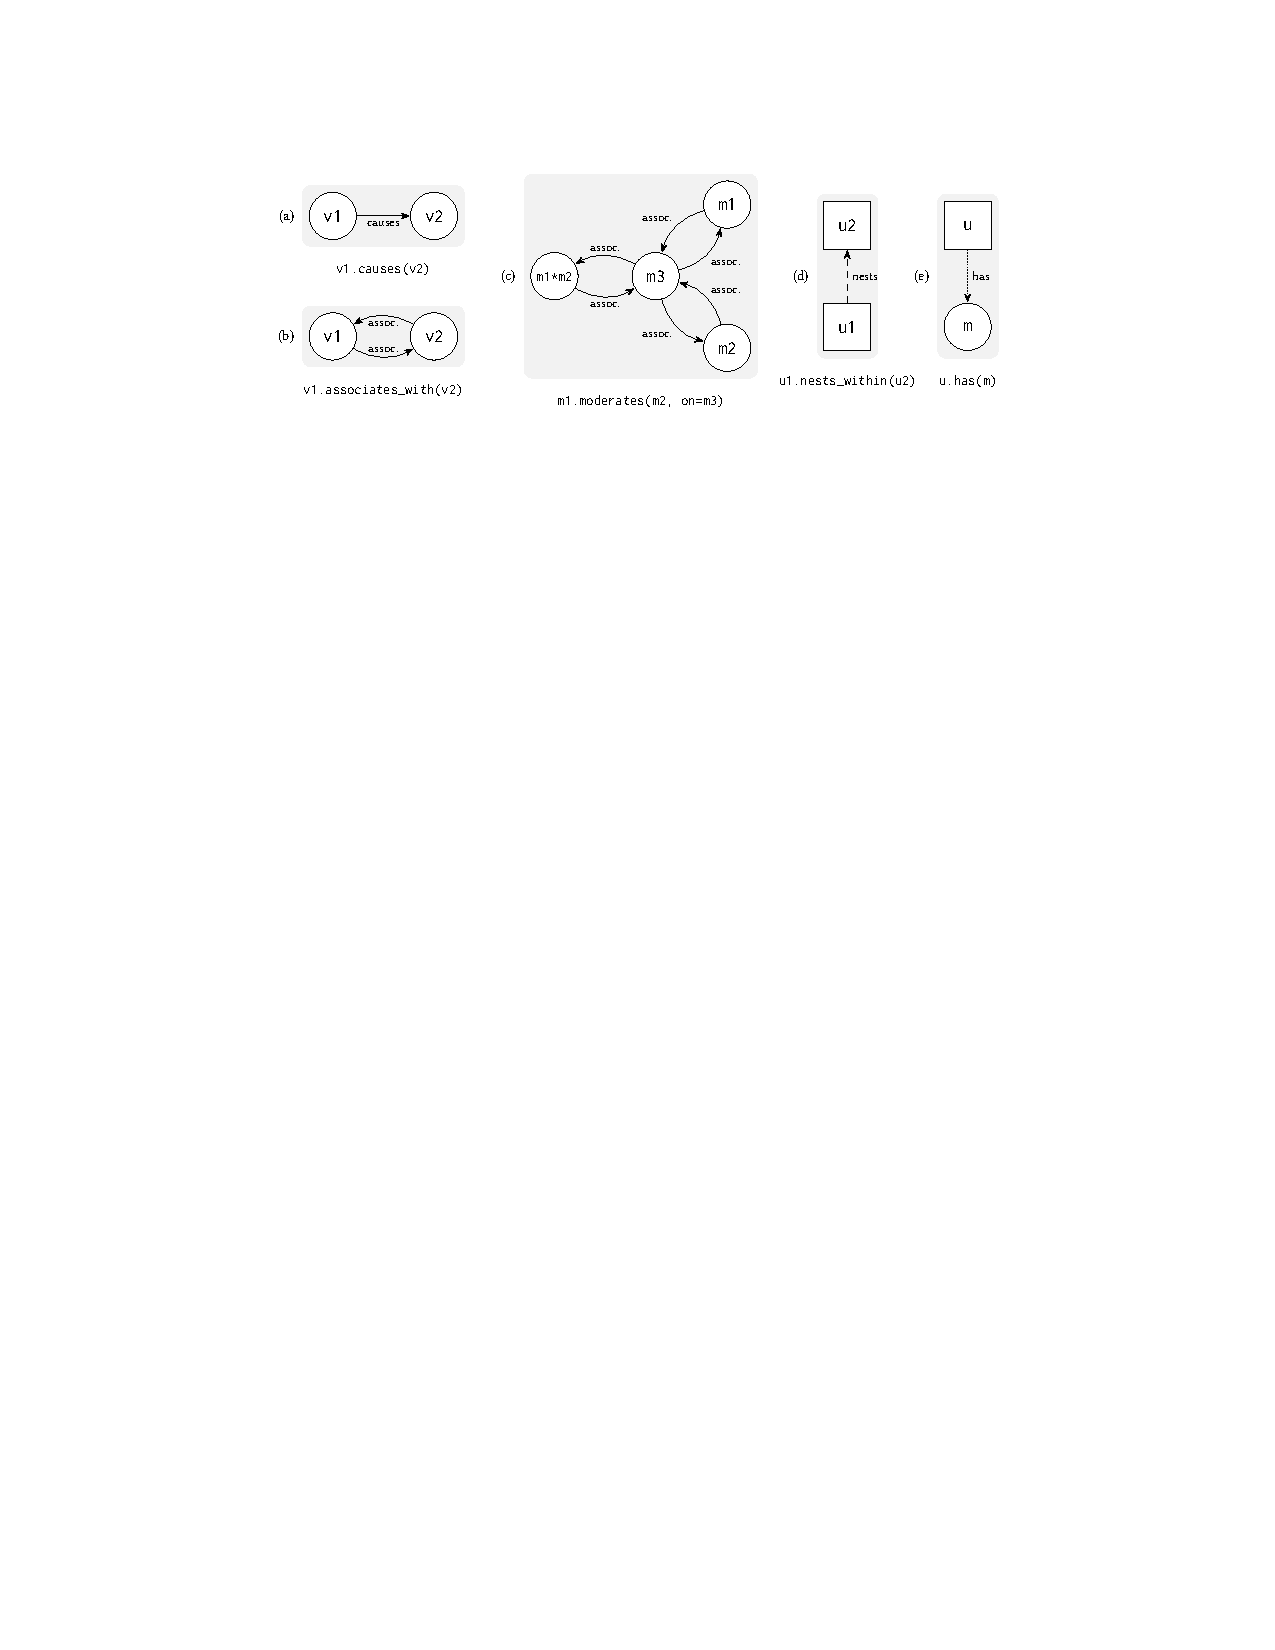
\includegraphics{tisane/figures/figure3}
%         \caption{Code snippets of conceptual and data measurement relationships written in Tisane's \SDSLlong and their representation in Tisane's graph IR. Variables are named with \texttt{u} for units, \texttt{m} for measures, and \texttt{v} for data variables that can be either units or measures. All edges depicted are those that are added due to the relationship. In the \texttt{moderates} example, we assume that \texttt{m1} and \texttt{m2} both belong to the same unit, and for simplicity, the attribution edge (labeled as ``has'') from \texttt{m1} and \texttt{m2}'s unit is not shown.}
%         \label{fig:figureSDSLToGraphIR}
%         \Description{Five directed graphs are shown. All nodes are labeled with a monospaced font. The first directed graph has two nodes, labeled “v1” and “v2”, both circles. There is a solid edge from “v1” to “v2” labeled “causes”. Below this graph is a code snippet reading “v1.causes(v2)”. The second directed graph also has two nodes, also labeled “v1” and “v2” and both circles. There are solid edges from “v1” to “v2” and from “v2” to “v1”. Both edges are labeled “assoc.” Below the graph is a code snippet: “v1.associates_with(v2)”. The third directed graph contains four nodes, which are labeled “m1*m2”, “m1”, “m2”, and “m3”. All are circles. There are six edges in the graph, all solid and labeled “assoc.” The edges are from “m1*m2” to “m3”, “m3” to “m1*m2”, “m1” to “m3”, “m3” to “m1”, “m2” to “m3”, and “m3” to “m2”. Below the graph is a code snippet: “m1.moderates(m2, on=m3)”. The fourth directed graph contains two nodes, labeled “u1” and “u2”. Both are squares. There is a dashed edge labeled “nests” from “u1” to “u2”. Below the graph is the code snippet “u1.nests_within(u2)”. The fifth, and final, directed graph contains two nodes labeled “u” and “m”. “u” is square-shaped and “m” is circle-shaped. There is a dotted edge from “u” to “m”, labeled “has”. Below the graph is the code snippet “u.has(m)”.}
%     \end{figure*}


\paragraph{Data measurement relationships.}\label{sec:data-measurement-relationships}

Study designs may have clusters of observations that need to be modeled explicitly for external validity.
For example, in a within-subjects experiment, participants provide multiple
observations for different conditions. An individual's observations may cluster
together due to a hidden latent variable. Such clustering may be imperceptible
during exploratory data visualization of a sample but can threaten external validity.
%(see~\ref{sec:validity}).
GLMMs can mitigate three common sources of clustering that
arise during data collection
~\cite{gelmanHill2006regression,kreft1998introducing,cohen1988statistical}:

\begin{itemize}
  \item \textbf{Hierarchies} arise when one observational/experimental unit
  (e.g., adult) nests within another observational/experimental unit (e.g.,
  group). This means that each instance of the nested unit belongs to one and
  only one nesting unit (many-to-one).
  % The nesting unit has multiple nested units.
  \item \textbf{Repeated measures} introduce clustering of observations from the
  same unit instance (e.g., participant).
  \item \textbf{Non-nesting composition} arises when overlapping attributes
  (e.g., stimuli, condition) describe the same observational/experimental unit
  (e.g., participant)~\cite{gelmanHill2006regression}.
\end{itemize}

The above sources of clustering pose three problems for analysts. First,
analysts must have significant statistical expertise to identify when data
observations cluster. Second, they must know how to mitigate these clusters in
their models. Third, with this knowledge, analysts must figure out how to
express these types of clustering in their analytical tools. Even if analysts
are not able to identify clustered observations, they are knowledgeable about
how data were collected.

% \enlargethispage{-12pt}

Thus, Tisane addresses the three problems by (i) eliciting data measurement
relationships from analysts to infer clusters and (ii) formulating the maximal
random effects structure, optimizing for external validity
(\autoref{sec:interaction_model}). Below, we describe language features for expressing data measurement relationships.

\paragraph{Nesting relationships: Hierarchies}
\textbf{Hierarchies} arise when a unit (e.g., an \adult) is nested within another
unit (e.g., an exercise \group). Researchers may collect data with
hierarchies to study individual and group dynamics together or as a side effect of
recruitment strategies. To express such designs, Tisane provides the
\texttt{nests\_within} construct. Conceptually, nesting is strictly between
observational/experimental units, so Tisane type checks that the variables
that nest are both Units. %Tisane assumes there are multiple nested units within a nesting unit.
In the graph IR, a nesting relationship is encoded as an edge between two unit
nodes (\autoref{fig:figureSDSLToGraphIR}(d)). There is one edge from the nested
unit (e.g., \adult) to the nesting unit (e.g., \group)~\footnote{The GitHub repo contains a gallery of examples that include nesting relationships.}.

\paragraph{Frequency of measures: Repeated measures, Non-nesting composition}
\def\numberofinstances{\texttt{number\_of\_instances}\xspace}
When a measure is declared through a unit, Tisane adds an
attribution edge (``has'') from a unit node to a measure node (\autoref{fig:figureSDSLToGraphIR}(e)).
A unit's measure can be taken one or more times in a study. The frequency of
measurement is useful for detecting repeated measures and non-nesting
composition. In \textbf{repeated measures} study designs, each unit provides
multiple values of a measure, which are distinguished by another variable,
usually time. \textbf{Non-nesting}~\cite{gelmanHill2006regression} composition
arises when measures describing the same unit overlap. For example, HCI researchers studying input devices might
design them to utilize different senses (e.g., touch, sight, sound).
Participants in the study may be exposed to multiple different devices, which
act as experimental conditions of senses. The conditions are intrinsically tied to the
devices, and participants can be described as having both conditions and
devices, which overlap with one another. Such study designs
introduce dependencies between observations~\cite{clark1973language} and hence
violate the assumption of independence that GLMs make.

\def\inputdevice{\texttt{device}\xspace} When analysts declare Measures, they
specify the frequency of the observation through the
\texttt{number\_of\_instances} parameter. This parameter accepts an integer,
variable, a Tisane \texttt{Exactly} operator, or a Tisane \texttt{AtMost}
operator. By default, the parameter is set to one. The \texttt{Exactly} operator
represents the exact number of times a unit has a measure. The \texttt{AtMost}
operator represents the maximum number of times a unit has a measure. Both
operators are useful for specifying that a measure's frequency depends on
another variable, which is expressible through the \texttt{per} function. For
example, participants may use two \inputdevice{}s \textit{per}
\texttt{condition} assigned: \texttt{device = subject.nominal(\upquote{Input
device}, number\_of\_instances=ts.Exactly(2).per(condition))}. \polish{Overruns column?} The \texttt{per}
function uses the Tisane variable's cardinality by default but can instead use a
data variable's \numberofinstances by specifying \texttt{use\_cardinality=False}
as a parameter to \texttt{per}. Moreover, specifying a measure's
\texttt{number\_of\_instances} to be an integer is syntactic sugar for using the
\texttt{Exactly} operator. Specifying a variable is syntactic sugar for
expressing \texttt{ts.Exactly(1).per(variable)}.

To determine the presence of repeated measures or non-nesting composition,
Tisane computes the \numberofinstances of measures and their relationship to
other measures. Measures that are declared with \numberofinstances equal to one
are considered to vary between-unit. Measures that are declared with
\numberofinstances greater than one or a variable with cardinality greater than
one are considered to vary within-unit as repeated measures. If there are
instances of a measure per another measure sharing the same unit, the measures
are non-nesting.

%     \begin{figure}[h]
% \centering
% 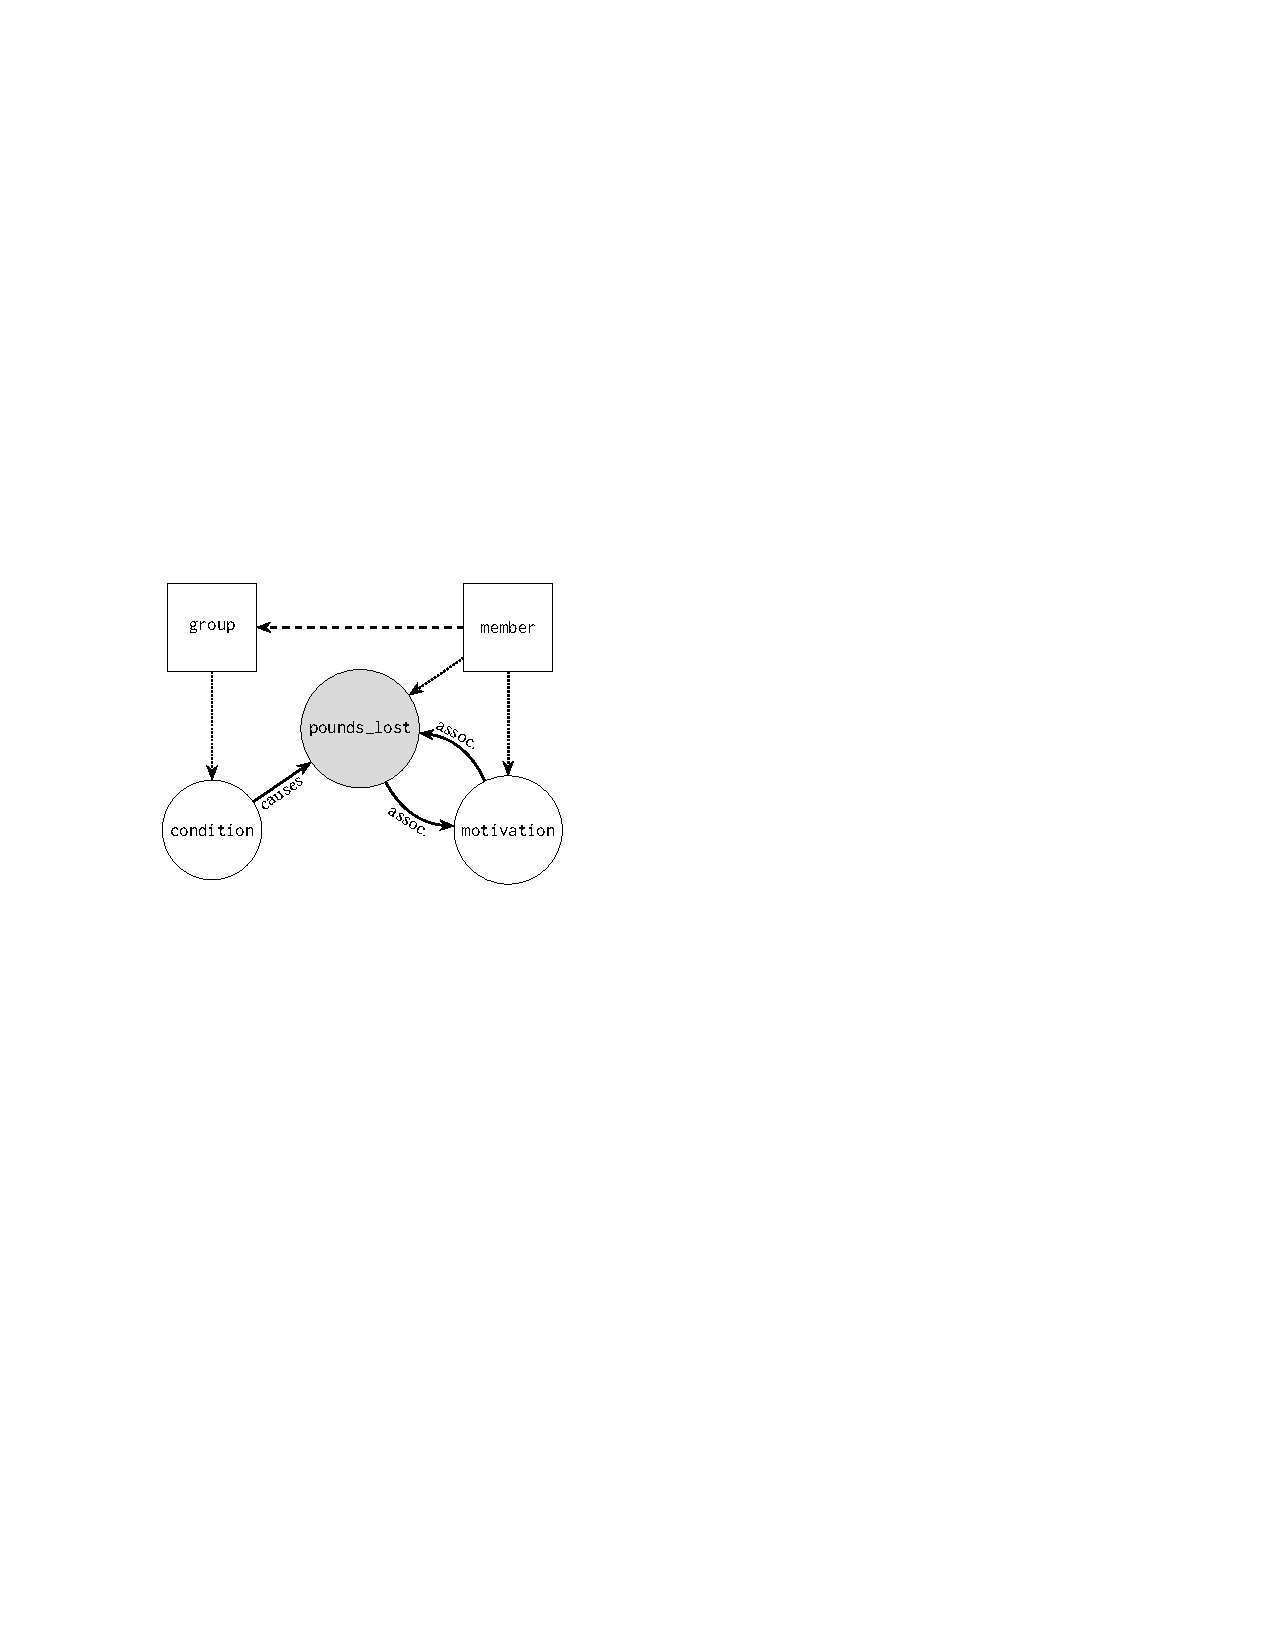
\includegraphics{tisane/figures/figure4}
%         \caption{The graph representation of the variables and relationships from the usage scenario. \texttt{causes} edges are labeled with ``causes''. \texttt{associates\_with} edges are labeled with ``assoc.'' Dashed edges indicate \texttt{nests\_within} relationships, and dotted edges indicate \texttt{has} relationships.}
%         \label{fig:figureGraphIRExample}
%         \Description{A directed graph of five nodes is depicted. The nodes are labeled “group”, “condition”, “pounds_lost”, “motivation”, and “member”, all in monospace font. The “group” node is square-shaped (indicating the node represents a Unit), and has a dotted edge pointing to the circle-shaped (indicating it's a Measure) “condition” node. The “condition” node has a solid edge labeled “causes” pointing to the circle-shaped, gray “pounds_lost” node. The gray color indicates that “pounds_lost” was the dependent variable. The “pounds_lost” node has one outgoing solid edge labeled “assoc.” (for associative relationships), to the circle-shaped node “motivation.” The “motivation” node has an outgoing, solid “assoc.” edges to the “pounds_lost” node. The final node, “member,” is square-shaped and has a dashed outgoing edge to the “group” node and dotted outgoing edges to the “pounds_lost” and “motivation” nodes. The dashed edge means “member” nests in “group” and the dotted edges mean that “pounds_lost” and “motivation” are measures of the “member” unit.}
%     \end{figure}

\subsection{Statistical Model Derivation: Interactively Querying the Graph IR}
\label{sec:interaction_model} After specifying variable relationships, analysts
can query Tisane for a statistical model. Queries are constructed by specifying
a study design with a dependent variable (the value to be predicted) and a set
of independent variables (predictors). Tisane processes the query and generates
a statistical model in four phases: (1) preliminary conceptual checks that
validate the study design, (2) inference of possible effects structures and
family and link functions, (3) input elicitation to disambiguate possible
models, and (4) generation of a final executable script, and a record of decisions during disambiguation. Given that the interactive process begins with
an input program using Tisane and outputs a script for fitting a GLM or GLMM, we
call this process \textit{interactive compilation}.

\subsubsection{Preliminary checks} \label{sec:prelim-checks}
At the beginning of processing a query, Tisane checks that every input study
design is well-formed. This involves two conceptual correctness checks. First,
every independent variable (IV) in the study design must either cause or be
associated with the dependent variable (DV) directly or transitively. Second, the
DV must not cause any of the
IVs, since it would be conceptually invalid to explain a
cause from any of its effects. If any of the above checks fail, Tisane
issues a warning and halts execution. By using these two checks, the Tisane
compiler avoids technically correct statistical models that have little to no
conceptual grounding (\dcConceptualKnowledge). If the checks pass, Tisane proceeds to the next phase.
% Tisane ensures that any statistical model it infers is both conceptually and
%technically valid relative to the analyst's specified relationships.

\subsubsection{Candidate statistical model generation}
A GLM/GLMM is comprised of a model effects structure, family function, and link
function. The model effects structure may consist of main, interaction, and
random effects. Tisane utilizes variables' conceptual relationships to infer candidate
main and interaction effects and data measurement relationships to infer
random effects. Tisane infers family and link functions based on the data type
of the DV in the query. The candidate statistical models that Tisane
generates, based on the graph and query, seed an interactive disambiguation
process.

The purpose of identifying candidate main effects beyond the ones analysts may
have specified is to provoke consideration of erroneously omitted variables that
are conceptually relevant and pre-empt potential confounding and
multicollinearity issues that may arise.

\paragraph{Deriving Candidate Main Effects}
In a query to infer a statistical model, analysts specify a single dependent
variable and a set of one or more IVs. After passing the checks described in~\autoref{sec:prelim-checks}, %As described above, the input IVs are
%checked to make sure that they have conceptually causal or associative %relationships. %Given that they do,
the query's independent variables are considered candidates. In addition, Tisane
derives three additional sets of candidate main effects intended to control for
confounding variables in the output statistical model\footnote{Tisane currently
treats each input IV as a separate ``exposure'' variable for which to identify
confounders. Tisane then combines all confounders into one statistical model.}.
The first two sets below are from the ``modified disjunctive cause
criterion''~\cite{vanderweele2019modifiedDisjunctiveCriterion}:

\begin{itemize}    
    \item \textbf{Causal parents.} For each IV in the query, Tisane finds its
    causal parents (see~\autoref{fig:figureCandidateMainEffects}(a)).
    % , as recommended
    % by~\cite{vanderweele2019modifiedDisjunctiveCriterion}.
    \item \textbf{Possible causal omissions.} Tisane looks to see if any other
    variables not included as IVs cause the DV 
    % , as recommended
    % in~\cite{vanderweele2019modifiedDisjunctiveCriterion} 
    (see
    in~\autoref{fig:figureCandidateMainEffects}(b)). They are relevant to the DV
    but may have been erroneously omitted.
    \item \textbf{Possible confounding associations.} For each IV, Tisane looks
    for variables that are associated with both the IV and the DV (see
    in~\autoref{fig:figureCandidateMainEffects}(c)). Because associations
    between variables can have multiple underlying causal structures, Tisane
    recommends variables with associative relationships with caution. Tisane
    issues a warning describing when not to include such a variable in the GUI.
\end{itemize}

\figureCandidateMainEffects

%     \begin{figure*}%[h]
% \centering
% 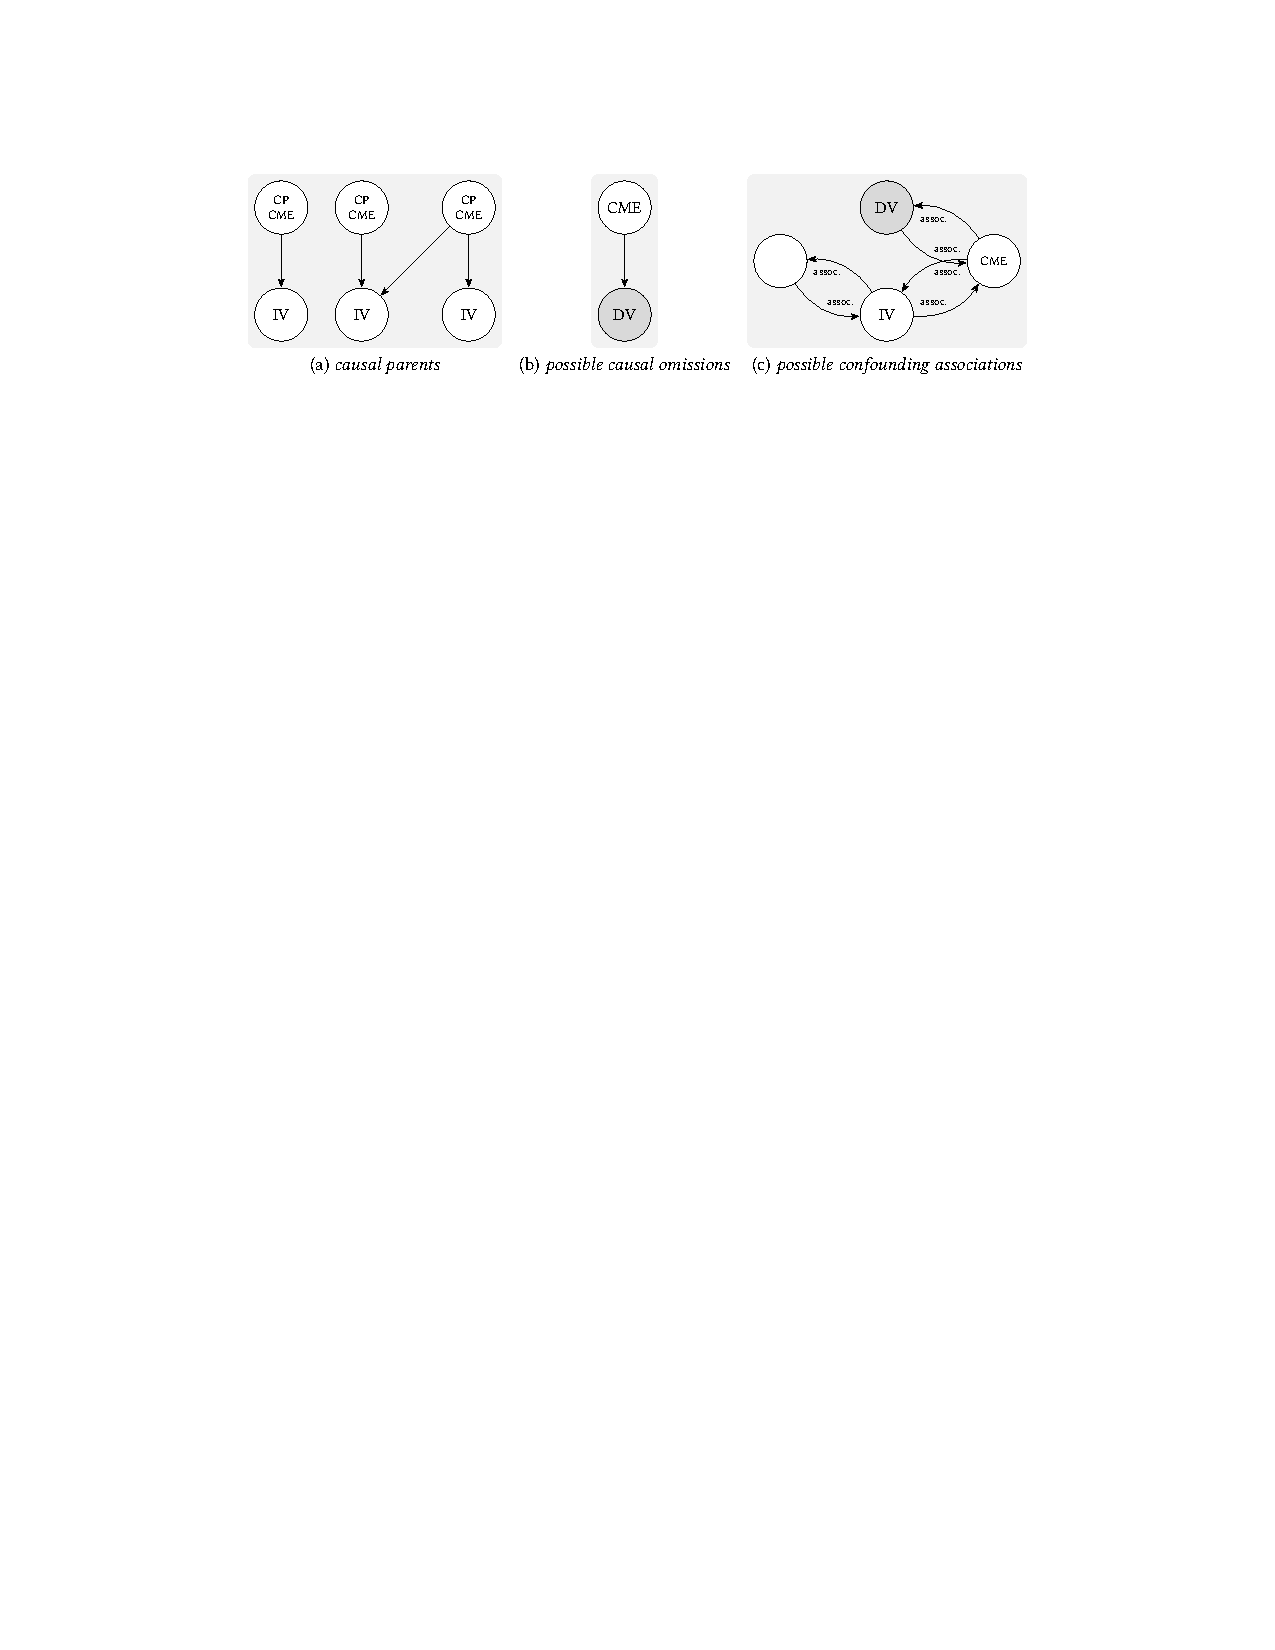
\includegraphics{tisane/figures/figure5}
%         \caption{Graphs demonstrating causal parents, possible causal omissions, and possible confounding associations. In graphs (a) and (b) (left and middle), all edges are causal. Independent variables are marked ``IV'', discovered candidate main effects ``CME'', dependent variables ``DV'', and causal parents ``CP''.}
%         \label{fig:figureCandidateMainEffects}
%     \end{figure*}

Using the above rules, Tisane suggests a set of variables that are likely
confounders of the variables of interest expressed in the query. There may be
additional confounders due to unmeasured or unexpressed variables that are either
not known or excluded from the graph. Tisane never automatically includes the
candidate main effects in the output statistical model. Analysts must always
specify a variable as an IV in the query or accept a suggestion (\dcGuidance).

If a graph only contains associates edges then the candidate main effects Tisane
suggests are those that are directly associated with both the DV and an IV. If a
graph has only causal edges, Tisane would suggest variables that directly cause
the DV but were omitted from the query and the causal parents of IVs in case the
parents exert causal influence on the DV through the IV or another variable that is not
specified.

The total set of main effects, including variables the analyst has specified as
IVs in their query and candidate main effects, are used to derive candidate interaction
effects and random effects, which we discuss next.

% However, relying on formal causal analysis to guide modeling is insufficient,
% and additional methods for ensuring conceptual validity are necessary.
\paragraph{Deriving Candidate Interaction Effects}
An interaction between variables means that the effect of one variable (the \textit{moderated} variable) on a \textit{target} variable is moderated by another (non-empty) set of variables (the \textit{moderating} variables). Tisane's
\SDSL already provides a primitive, \texttt{moderates}, to
express interactions. As such, Tisane's goal in suggesting candidate interaction
effects is to help analysts avoid omissions of conceptual relationships
that are pertinent to an analyst's research questions or hypotheses (\dcConceptualKnowledge).
Candidate interaction effects are the interaction nodes whose (i) moderated and moderating variables include two or more candidate main effects and (ii)
    target variable is the query's DV.

\paragraph{Deriving Candidate Random Effects} \label{sec:deriveRandomEffects}
Random effects occur when there are clusters in the data, which occur when
we have repeated measures,
nested hierarchies, or non-nesting composition (as defined in~\autoref{sec:data-measurement-relationships}). Tisane implements Barr et al.'s recommendations
for specifying the maximal random effects structure of linear mixed effects
models for increasing the generalizability of statistical
results~\cite{barr2013random, barr2013randomUpdated}.

To derive random effects, Tisane focuses on the data measurement edges in the
graph IR. Using the graph IR, Tisane identifies unit nodes, looks for any nesting
edges among them, and determines within- or between-subjects
measures based on the frequency of observations for units. % by using metadata stored in the attribution edges about the number of
%observations each unit has of any particular measure.
From these, Tisane
generates random intercepts of units for the unit's measures that are between-subjects as well as the unit's measures that are within-subjects where each instance of the unit
has only one observation per value of another variable. Tisane generates random slopes of a unit and its measure for all measures
that are within-subjects where each instance of the unit has multiple
observations per value of another variable. For interaction effects, random
slopes are included for the largest subset of within-subjects variables (see~\cite{barr2013randomUpdated}). %,
%according to Barr's updated recommendations~\cite{barr2013randomUpdated}.
Tisane handles correlation of random slopes and intercepts during disambiguation (\autoref{sec:disambiguation}).
%When there are both random slopes and random intercepts for the same unit, Tisane asks analysts if they are correlated during disambiguation. By default, Tisane assumes correlation.
% due to computational limitations or insufficient data,
Maximal random effects may lead to model convergence issues that analysts
address by later removing or adding independent variables and random effects. Nevertheless, starting with
a maximal, valid model is important for ensuring that future revisions are also valid (\dcValidity).

\paragraph{Deriving Candidate Family and Link Functions} \label{sec:family_link_functions}
\tableFamilyLinkFunctions
The DV's data type determines the set of candidate family and
link functions. For example, numeric % or continuous data
variables cannot have
binomial or multinomial distributions. Similarly, nominal variables are not
allowed to have Gaussian distributions. Furthermore, each family has a set of
possible link functions. For example, a Gaussian family distribution may have an
Identity, Log, or Square Root link function. The statistics literature documents
    possible combinations of family and link functions for specific data
types~\cite{nelder1972generalized}.
%  that software tools such as
% statsmodels~\cite{statsmodelsRef} and lme4~\cite{bates2014fittingLme4}
% implement.

Tisane includes common family distributions as candidate families and their
applicable link functions. In its current implementation, Tisane relies on
\statsmodels~\cite{statsmodelsPaper} for GLMs and
\texttt{pymer4}~\cite{jolly2018pymer4} for GLMMs. As such, Tisane is limited to
the family and link function pairings implemented in these
libraries.~\autoref{tab:tableFamilyLinkFunctions} lists the family and link
functions these libraries currently supports. As \statsmodels' and \pymer's
support for GLMs grows in the future, Tisane can be extended.
% Tisane can be
% extended to take advantage of new family and link implementations in these
% libraries.



\subsubsection{Eliciting Analyst Input for \Disambiguation}\label{sec:disambiguation}
% Upon generating a set of candidate main, interaction, and random effects, Tisane
% asks analysts questions before outputting a statistical model.
The disambiguation process provides an opportunity for analysts to explore the
space of generated models based on their original query. Given our design
considerations to prioritize conceptual knowledge (\dcConceptualKnowledge) and
give analysts guidance (\dcGuidance), we designed a GUI to scaffold analysts' reasoning and elicit their input.
For versatility, we implemented Tisane's GUI using Plotly
Dash~\cite{plotlyDash}. Analysts can either execute their Tisane programs and use the
GUI inside a Jupyter notebook (no additional widgets needed) or run
their Tisane programs in an IDE or terminal, in which case Tisane will open the
GUI in a web browser. 

\groupExerciseDisambiguation
% Figure~\ref{fig:groupExerciseDisambiguation}
% gives an overview of the GUI.

% Tisane grounds explanations and disambiguation questions in the
% variable relationships analysts declared in their input Tisane program,
% for explaining why specific generated main and interaction effects may be
% desirable, how Tisane automatically inferred the random effects structure, and
% show data distributions to help analysts select family and link functions (Figure~\ref{fig:groupExerciseDisambiguation}).
Candidate statistical models are organized according to (i) independent
variables  (main effects and interaction effects), (ii) data clustering (random
effects), and (iii) data distribution (family and link functions). In the main
effects tab, Tisane asks analysts if they would like to include additional or
substitute main effects that Tisane infers to be conceptually relevant. In the
interaction effects tab, Tisane suggests moderating relationships to include but
does not automatically include them because analysts may not have specific
hypotheses involving interactions (\dcGuidance). If analysts do not specify any
moderating relationships, Tisane does not suggest any interaction effects,
preventing analysts from including arbitrary interactions that may be
conceptually unfounded (\dcConceptualKnowledge, \dcValidity).

In the data clustering tab, Tisane shows analysts which random effects it
automatically includes based on the selected main and interaction effects. Unlike
main and interaction effects, Tisane automatically includes random effects
in order to maximize model generalizability (\dcValidity). If there is a random
slope and random intercept pertaining to the same unit, Tisane asks analysts if
they should be correlated or uncorrelated. We provide this option because
analysts may have relevant domain expertise to make this decision (\dcGuidance).
By default, Tisane correlates the random slope and random intercept.

The final tab, data distribution, helps analysts examine their data and select
an initial family and link function to try. Appropriate selection of family and
link functions depends on the data type of the dependent variable and the
distribution of model residuals. Therefore, the selection can only be assessed
after choosing a family and link function in the first place.

For an initial statistical model to consider, Tisane narrows the set of family
functions considered based on the declared data type of variables
(see~\autoref{sec:family_link_functions}) and lightweight viability checks, such
as ensuring that a Poisson distribution is only applicable for variables that
have nonnegative integer values. Tisane asks questions designed to uncover
more semantically meaningful data types (e.g., counts) than are provided at
variable declaration. Analysts without data can answer these questions as they
are planning their studies (\dcStatisticalPlanning). For the selected family
candidate, Tisane automatically selects the default link function based on the
defaults for \statsmodels~\cite{statsmodelsRef} and
\texttt{pymer4}~\cite{jolly2018pymer4}. Analysts can then choose a different
link function, as long as it is supported.
% \footnote{See supplemental material for
% a complete listing of Tisane's supported family and link function pairings.}.}
% We chose to ask these questions during
% disambiguation rather than provide additional data types to Tisane's \SDSL to
% simplify the variable declaration process. \ej{Not sure I believe this.}}

\subsubsection{Output}
There are two outputs of the interactive compilation: (ii) an executable modeling script and (ii) a log of GUI
choices. To increase transparency of the
authoring process, Tisane provides a log of user selections in the GUI as
documentation, which the analyst can include in pre-registrations, for example
(\dcStatisticalPlanning). In the output script, Tisane includes code to fit the
model and plot residuals against fitted values in order to assess the
appropriateness of family and link functions, as is typical when examining
family and link functions. The output script also includes a comment explaining
what to look for in the plots and an online resource for further reading. Should
analysts revise their choice of family and link functions, they can re-generate
a script through the Tisane GUI.